\chapter{Methodology}
This chapter will outline the steps needed and the choices made for this project to implement a successful CNN.
\section{Data Selection}
The first point for considering what dataset to use for this project was to identify an open-source product and with a resolution of less than one metre. It had to comprise of an RGB image with an associated mask layer representing the feature or features of interest. In \cite{Richmond19b}, Table \ref{tab.datasets} displays all the datasets that were considered with justifications for each. For this thesis the INRIA Building Dataset was used, this dataset was developed for the project outlined in \cite{maggiori17a}. Their dataset was created to ensure it contained recent orthorectified imagery; recent official cadastral records; precise registration between orthorectified imagery and cadastral records; open-access data, for both imagery and cadaster; and coverage that varied across urban landscapes and illumination. \cite{maggiori17a} found that there were certain areas in Austria and the US that satisfied these requirements and they focused on zones where reference data and images were available. The US imagery was provided at either 15 or 30cm resolutions with three to four spectral bands and the Austrian data contains three bands at a resolution of 10 or 20 cm. They built the dataset to be consistent at 30 cm and RGB by using average re-sampling where needed. For there feature mask they considered two classes, \textit{building} and \textit{not building}. Subsequently, they visually inspected the imagery to ensure the cadaster datasets were properly aligned with the imagery, removing cities where irregular shifts had occurred. 

\begin{table}[htpb]
\centering
\begin{adjustbox}{width=1\textwidth,center=\textwidth}
\begin{tabular}{l|llll|ll}
\textbf{Train}      & Tiles* & Total area &  & \textbf{Test}       & Tiles* & Total area \\ \cline{1-3} \cline{5-7} 
Austin, TX          & 36     & 81 km$^2$     &  & Bellingham, WA      & 36     & 81 km$^2$     \\
Chicago, IL         & 36     & 81 km$^2$     &  & San Francisco, CA   & 36     & 81 km$^2$     \\
Kitsap County, WA   & 36     & 81 km$^2$     &  & Bloomington, IN     & 36     & 81 km$^2$     \\
Vienna, Austria     & 36     & 81 km$^2$     &  & Innsbruck, Austria  & 36     & 81 km$^2$     \\
West Tyrol. Austria & 36     & 81 km$^2$     &  & East Tyrol, Austria & 36     & 81 km$^2$     \\
Total               & 180    & 405 km$^2$    &  & Total               & 180    & 405 km$^2$   
\end{tabular}
\end{adjustbox}
\caption[Dataset statistics.]{Dataset statistics. *Tile size:1500$^2$ px. (0.3m resolutions) taken from \cite{maggiori17a}.}
\label{tab.inria_dataset}
\end{table}

Table \ref{tab.inria_dataset} depicts the regions included in the datasets and their distribution between training and test subsets. The dataset was split in evenly between training and test to allow for a proper assessment of the methods and how they can generalise to other areas. It was also split to ensure that each subset contained American and European examples as well as high-density urban areas (Chicago/San Francisco and Vienna/Innsbruck) and low-density (Kitsap/Bloomington and West/East Tyrol). \cite{maggiori17a} even made sure that some of the groups contained dissimilar information (e.g. the image from Kitsap County was taken from different flights with different characteristics). They created the reference data by rasterizing the cadastral shapefiles using GDAL and examples can be found in Figure \ref{fig.inria_dataset}.

\begin{figure}[htpb]
    \centering
    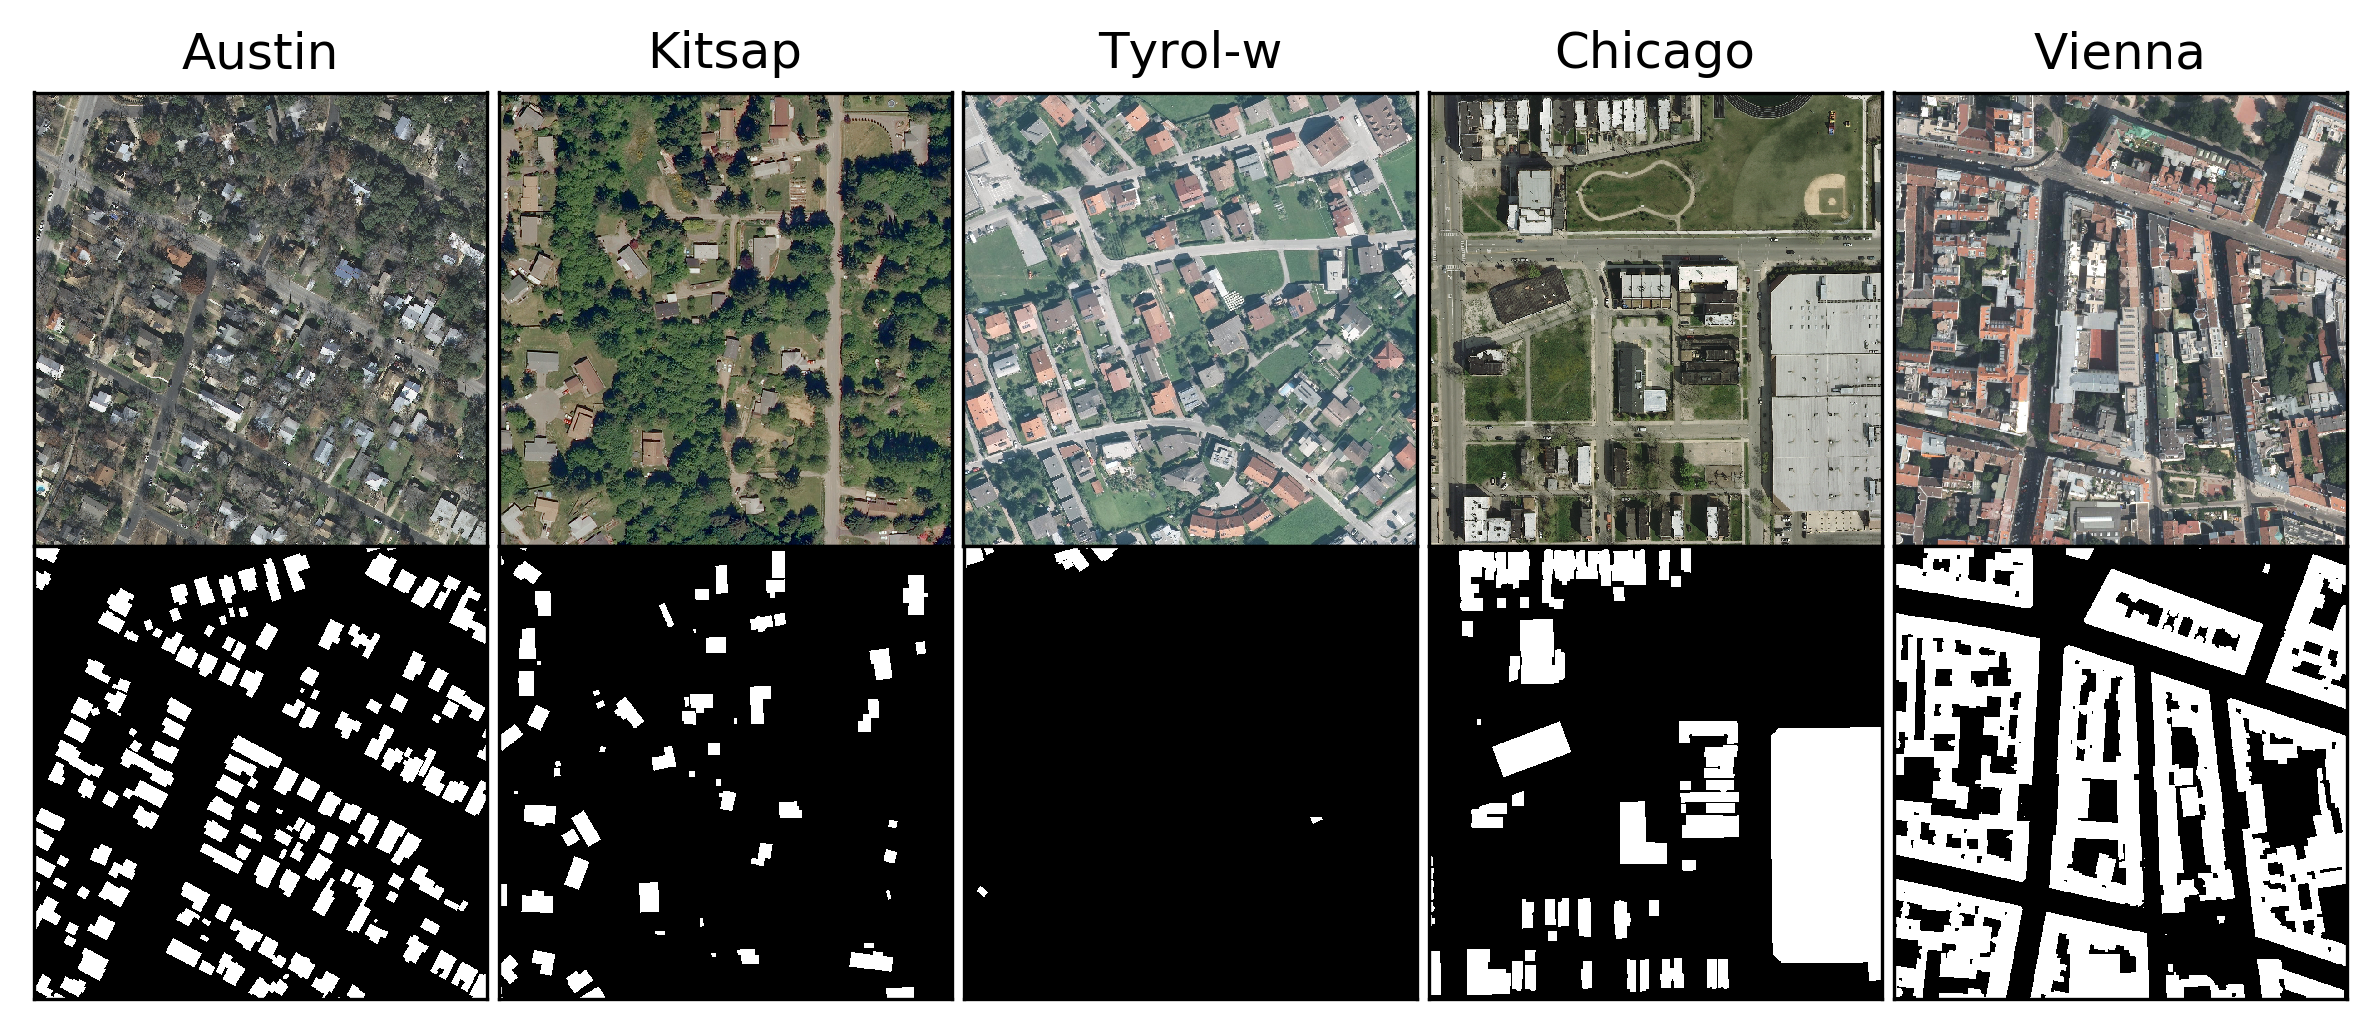
\includegraphics[width=1\textwidth]{\dir/figs/example_inria.png}
    \caption[Examples from the INRIA Image Labelling Dataset]{Example of individual tiles from the training dataset and their corresponding reference data. Images show a cutout of the full tiles, 1000 x 1000 px.}
    \label{fig.inria_dataset}
\end{figure}

\section{Model Architecture}\label{sec.model_architecture}
This section will discuss the architecture of the CNN and justify why certain elements were chosen over others, for a more detailed discussion of how CNNs work please refer to \cite{Richmond19b}.
\subsection{Convolutional Layer}
As this project aims to generate a framework that can be reusable by other researchers, the network has been generalised to work with any RGB image that has an associated binary mask. CNNs are made up of a series of convolutional (Conv) layers that work sequentially to transform the dimensions of the data. These Conv layers are the building blocks of the network and the designer of the network can adjust the number of Conv layers to transform the data more or less before a prediction is made on the class of the pixel. Each Conv layer accepts a volume of size\textbf{ $W_1\times H_1\times D_1$} and there are a series of hyperparameters that can be adjusted: the number of filters \textbf{K}, the spatial extent \textbf{F}, the stride \textbf{S}, and the amount of zero padding \textbf{P}. These transform the input volume so that \textbf{$W_2\times H_2\times D_2$} becomes: 
\[\textbf{$W_2 = (W_1 - F + 2P)/S + 1$}\] \[\textbf{$H_2 = (H_1 - F + 2P)/S + 1$}\]\[\textbf{ $D_2 = K$}\]
The typical hyperparameters for a CNN are $F = 3$, $S = 1$, $P = 1$, however, there are common conventions that motivate these hyperparameters. As remote sensing typically works with at least three channels in the input volume the generalised architecture structure here differs from common convention, the main difference being there are no Pool layers (this is discussed in more detail in \citet{Richmond19b}). This means a different set of hyperparameters were chosen for this specific project, $F = 4$, $S = 2$, $P = 1$. 
\subsection{Batch Normalisation}
Along with convolving the data in each block, the data goes through batch normalisation and an activation function. \citet{ioffe15} were the first to recognize the effect of internal covariate shift in deep learning problems. The effect of internal covariate shift is not significant within a single training set. But, if the trained network were to be applied to another region, the effect can result in an inaccurate model. In the CNN presented here, a batch normalisation function is applied to the batch and is separated from the optimiser and the gradient descent, this allows for higher learning rates in the network (Figure \ref{fig.batchnorm}). By normalising activations throughout the network, small changes to the parameters are prevented from amplifying into sub-optimal changes in the activation gradients (\cite{ioffe15}). 

\begin{figure}[htpb]
    \centering
    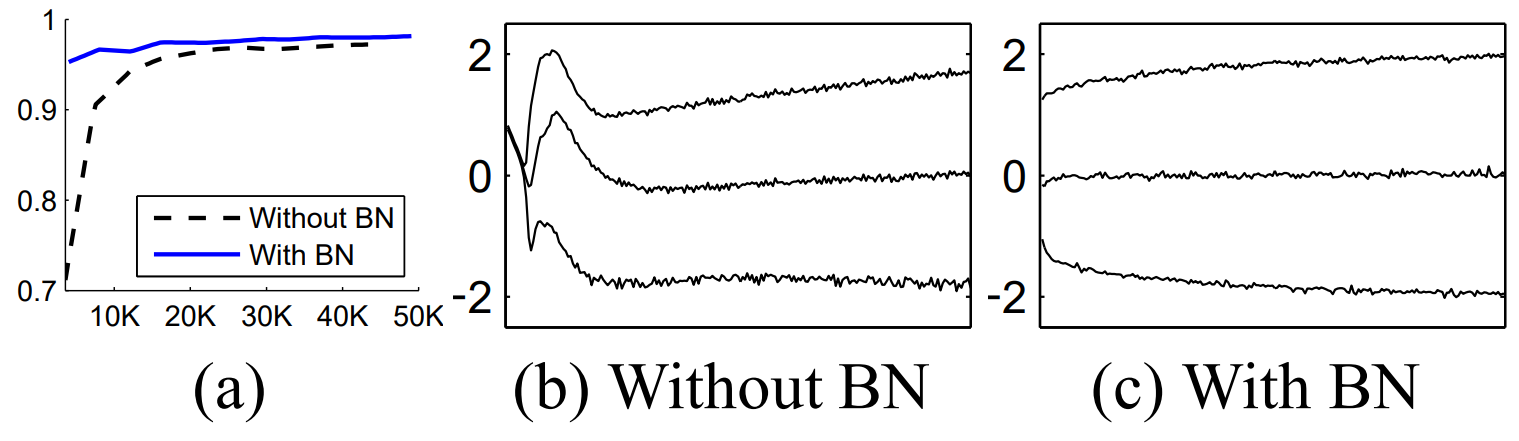
\includegraphics[width=0.75\textwidth]{\dir/figs/batchnorm.PNG}
    \caption[Example of the effect of Batch Normalisation]{Example of the effect of Batch Normalisation; (a) shows the test accuracy with and without Batch Normalisation plotted against the number of training steps. (b,c) Batch Normalisation makes the distribution more stable and reduced the covariate shift. Taken from \citet{ioffe15}.}
    \label{fig.batchnorm}
\end{figure}
\subsection{Activation Function}
Following normalisation, an activation function is applied to the input volume. The activation function introduces non-linearity to the network and converts the input signal to an output one for the next block in the architecture. Without an activation function the network would be a linear function and be limited in complexity and function. A CNN without an activation function, is simply a linear regression model. There are several different activation functions, all for different applications. The function used in this architecture is the Rectified Linear Unit (ReLU), which is the most reliable and can be used as a good approximation for all applications (\cite{krizhevsky17}). ReLu corrects a value to be 0 when $<$ 0 and then linear with a slope of 1 when x $>$ 0 (Figure \ref{fig.reluA}). 
\par

\begin{figure}[htpb]
    \centering
    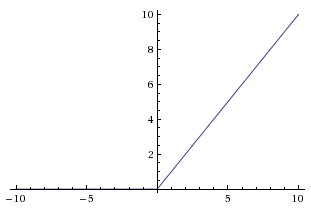
\includegraphics[width=0.5\textwidth]{Part2/chapter3/chapter/figs/relu.jpeg}
    \caption{ReLu function.}
    \label{fig.reluA}
\end{figure}
\subsection{Overall Architecture}
A CNN is split up into two sections, the encoder and the decoder. The encoder abstracts the data, predicts pixel class and then the decoder returns this prediction to the original resolution. The two parts of a CNN can be seen in Figure \ref{fig.unet_large}, on the left there is the encoder and on the right is the decoder. On either side of the figure, each Conv block transforms the dimensions of the input volume, either to convolve or deconvolve. For our architecture the output volume has two channels, if we were looking at multiple classifications this would increase relative to the number of classes. In our case, this is \textit{building} and \textit{non-building}. 

\begin{figure}[htpb]
    \centering
    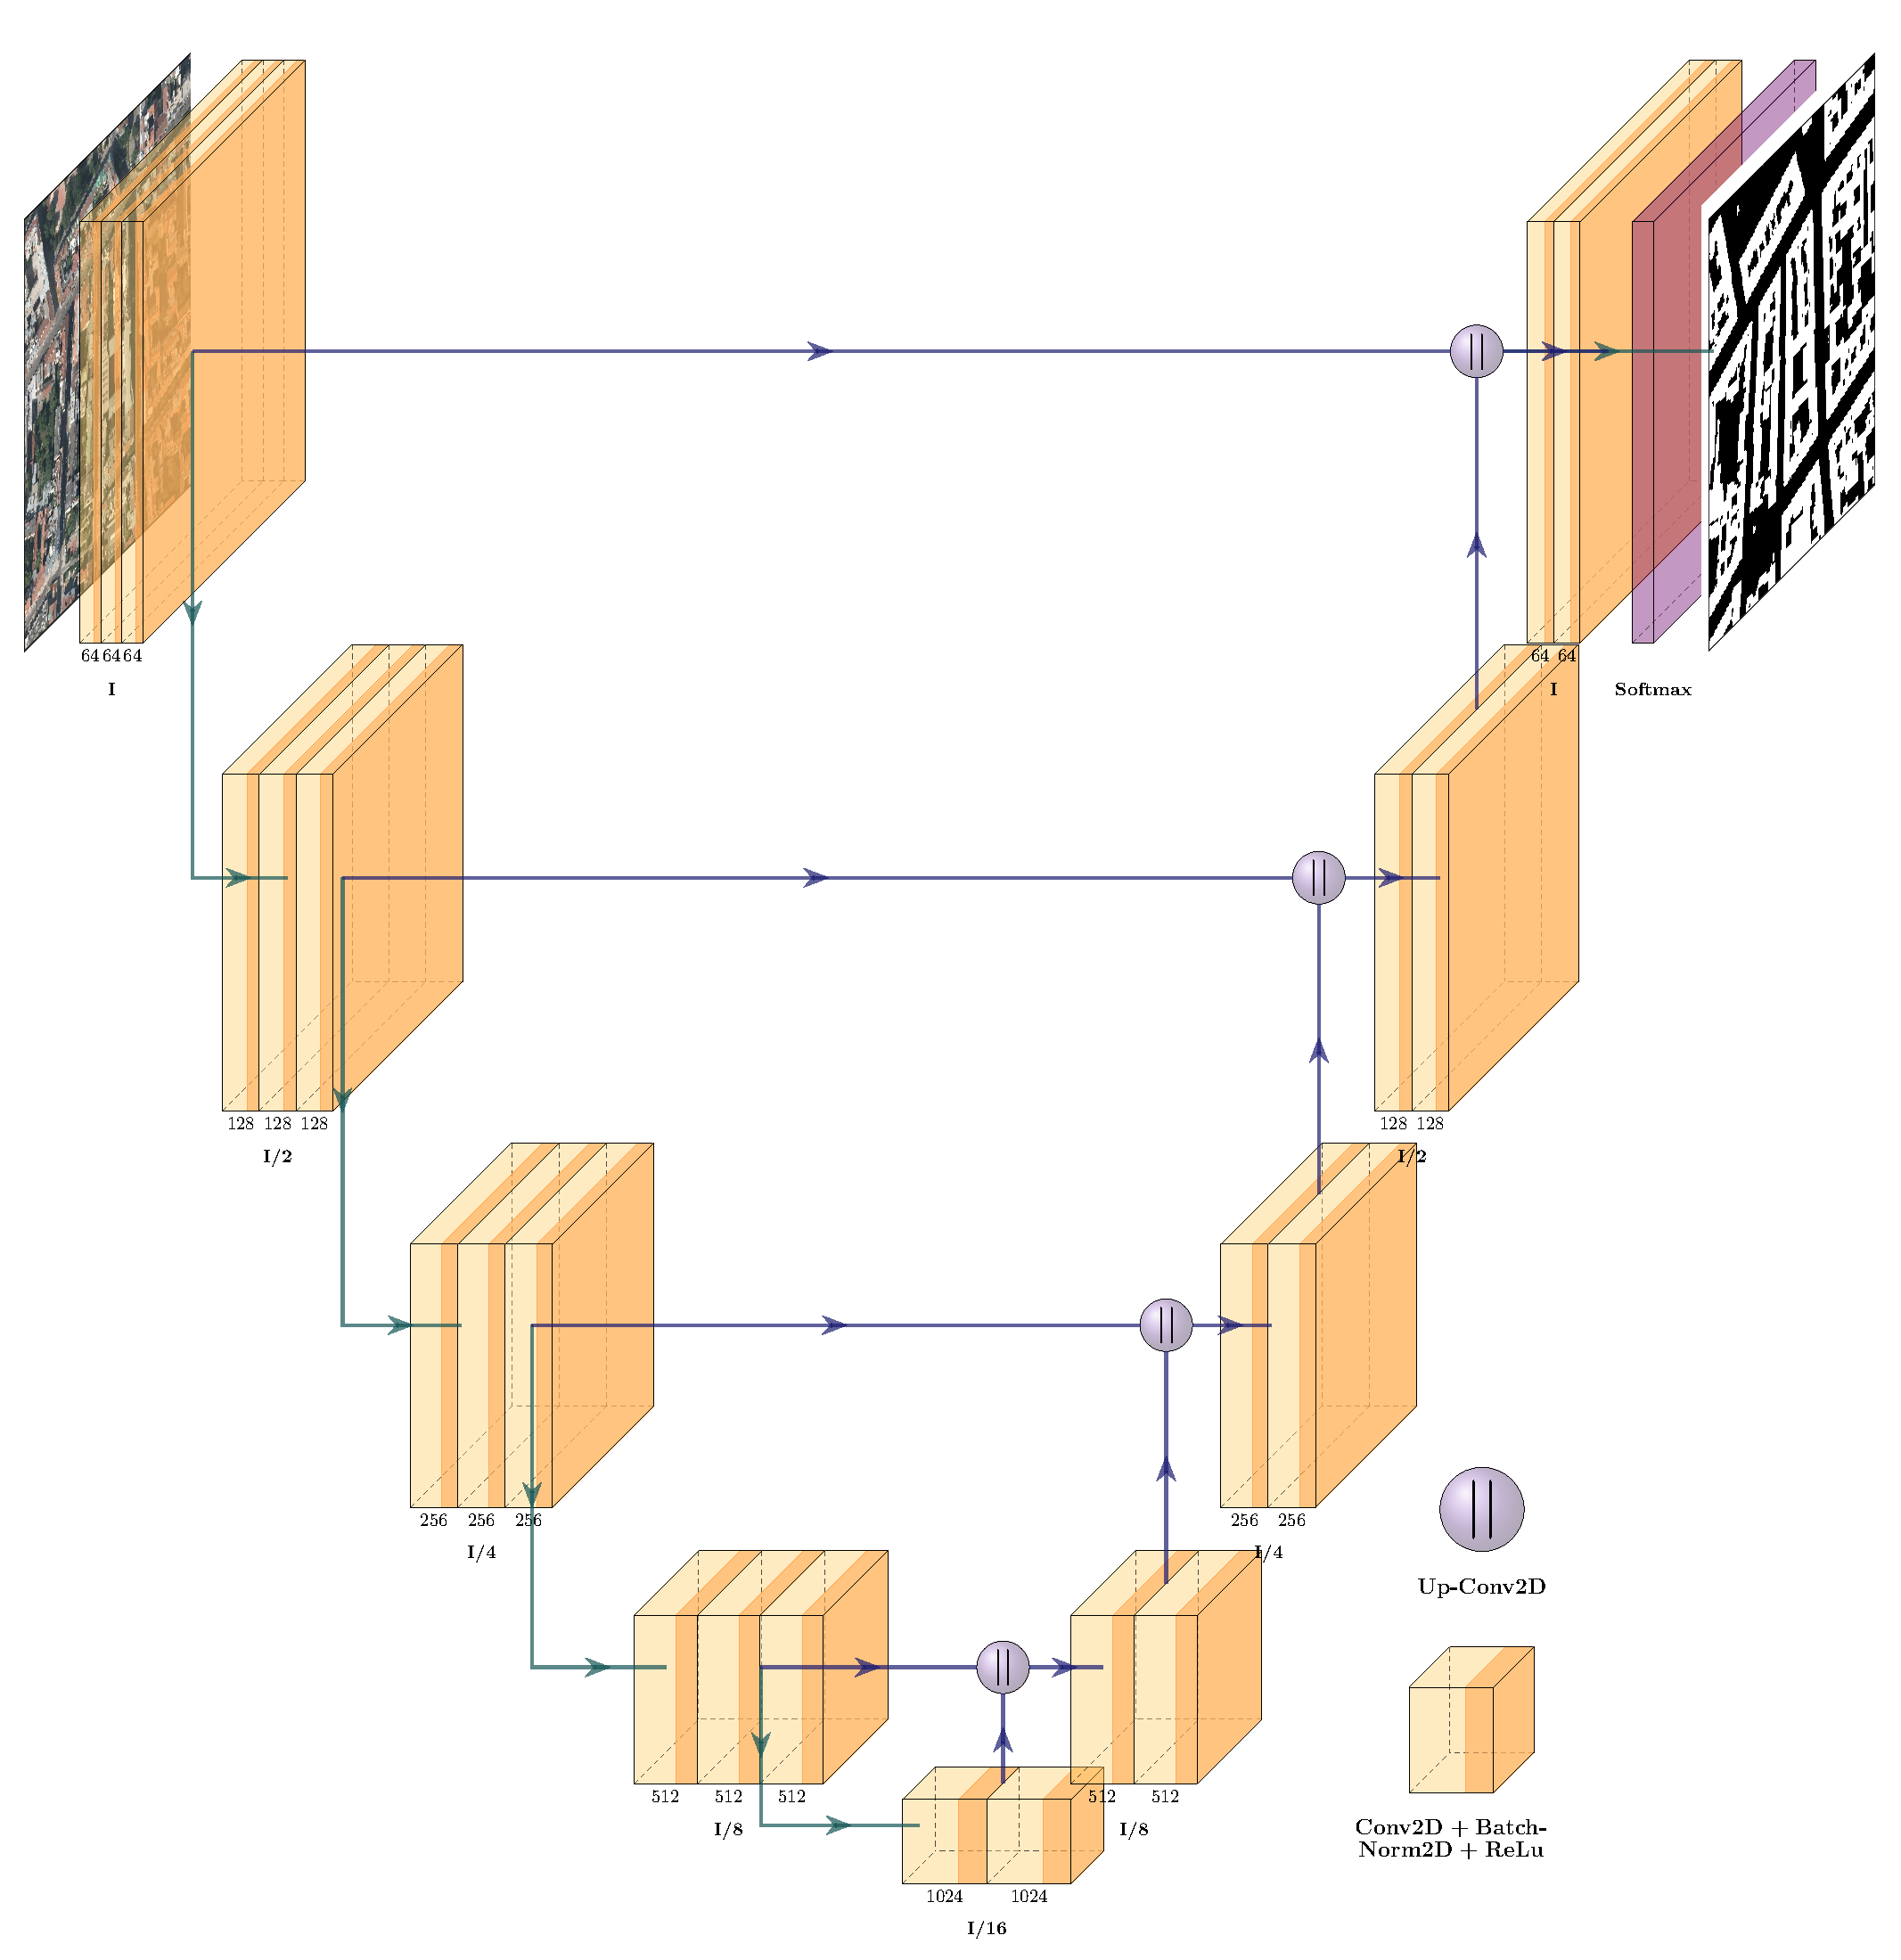
\includegraphics[width=1\textwidth]{\dir/figs/Unet_ushape.pdf}
    \caption[Schematic representation of the U-Net part of the network]{Schematic representation of the U-Net part of the network. Model ingests a three-channel RGB image and output a two-channel binary classification.}
    \label{fig.unet_large}
\end{figure}


\section{Model Training}\label{sec.model_training}
To begin training the model, the training dataset must first be split into training, validation and testing. This is done by an 60:20:20 split of all the data in the training set. During model training, the CNN will not touch the test set, this is to test the overall accuracy of the network. A successful model is one that achieves high accuracy in a relatively short amount of time. The training can be monitored by inspecting the loss rate as the training progresses. The data loss measures the compatibility between a prediction and the ground truth label. It is necessary to plot both the training loss and the validation loss as training progresses. 

% Typically validation loss should be similar to but slightly higher than the training loss once the training is concluded. As long as the validation loss is lower than or even equal to the training loss one should continue training the network. If the training loss reduced without an increase in validation loss, training continues. Once validation loss starts to increase, then the training should stop and the accuracy of the network evaluated. If the accuracy is not acceptable, then the model's parameters should be adjusted. 
\begin{figure}[htpb]
    \centering
    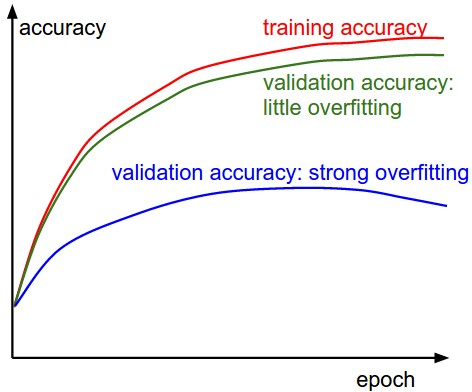
\includegraphics[width=0.5\textwidth]{\dir/figs/accuracies.jpeb}
    \caption[Examples of accuracy during training]{Examples of accuracy during training, the gap between the training and validation accuracy indicates the amount of overfitting.}
    \label{fig.accuracies}
\end{figure}
\subsection{Adjusting Model Parameters}
To test which combination of hyperparameters produces the best loss rate, many training runs need to be implemented to test all possible combinations. For the model presented here, the learning rate, batch size and the number of filters in the Conv layer were iterated over to see which produced the best loss rate and model accuracy over 100 training runs. The loss rate should be as close to the best case example in Figure \ref{fig.accuracies}, the combinations that produce the best loss rate will then be used to train the network over an increased number of epochs.
\subsubsection{Number of Filters in the Conv Layers}
As mentioned in Section \ref{sec.model_architecture} the number of filters in the Conv layer controls the depth to which the input is transformed as it is output to the next layer. The number of filters determines the number of feature maps that are produced during each convolution to represent the features in the image that is being analysed. It also contributes the amount of memory that the training will need and as the initial number of filters increases so does the amount of memory required. Adjusting the initial number of filters is a compromise between efficiency and accuracy. 

\subsubsection{Optimiser and Learning Rate}
The loss of the network is used to measure the error between the predicted output and the actual output. The network here used a Softmax classifier that uses cross-entropy to determine the loss. More detail on how the Softmax classifier works can be found in \citet{Richmond19b}. Optimisation finds the particular set of weights that work together to minimise the loss function (\cite{Karpathy_opt}). It is possible to calculate the best direction along which the weight vector should be changed to produce the steepest gradient for the loss to reach zero. However, it is not possible to determine the length of the steepest gradient section. Therefore the user needs to determine the step size, or learning rate after each iteration (\cite{Karpathy_opt}). For large scale neural networks this is calculated over the size of the batch rather than the entire training set and is often denoted as the Stochastic Gradient Descent (SGD) (\cite{Bottou98,Sutskever13}.
\par 
The optimiser used for this study is the \textit{Adam} optimiser. It was created as an algorithm that is well suited to handling large data problems, such as the ones proposed by the remote sensing community. It works by combining two popular algorithms AdaGrad (\cite{duchi11}) and RMSProps (\cite{tielman12}), and optimises the learning rate so that it anneals over time (\cite{kingma14}). The hyperparameters have intuitive interpretations and typically require little tuning, see \citet{kingma14}. In Figure \ref{fig.adam}, it is clear that the \textit{Adam} optimiser shows better convergence than other algorithms.

\begin{figure}[htpb]
    \centering
    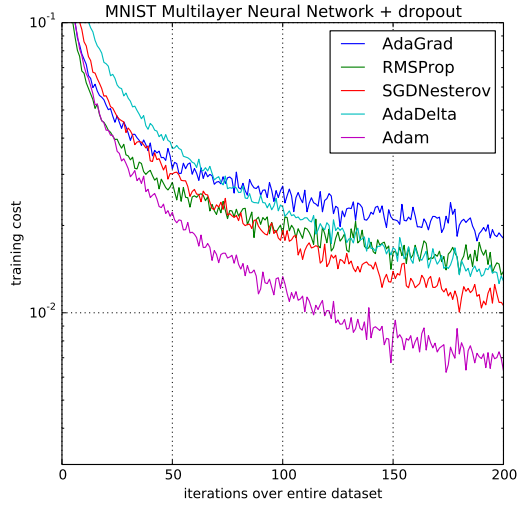
\includegraphics[width=0.8\textwidth]{\dir/figs/adam.PNG}
    \caption[Comparison of different optimisers]{Comparison of different optimisers, the lines depict how the cost of the various algorithms on the training. Taken from \citet{kingma14}}.
    \label{fig.adam}
\end{figure}
\subsubsection{Batch Size}\label{sec.batch_size}
The batch size determines the number of training samples that are utilised in one iteration (\cite{mnih13}). Stochastic Gradient Descents (SGDs) are employed in small-batch regimes where the batch size is typically less than the number of training samples. SGDs are limited for parallelisation due to the sequential natures of iterations, speed-ups are limited by the small batch size (\cite{simonyan14,,mnih13}). However, researchers have observed that this can lead to a loss in generalisation performance (\cite{Keskar16}), which is where the network is intended to perform best. 
\par
Fluctuations in the loss rate are caused by the batch size. When the batch size is 2 (Figure \ref{fig.min_batch}) the fluctuations will be relatively high. When the batch size is the full dataset (Figure \ref{fig.max_batch}), the fluctuations will be at their minimum because every gradient update should improve the loss function unless the gradient is too high (\cite{Karpathy3}). 


\begin{figure}[htpb]
\centering
\begin{subfigure}{0.45\textwidth}
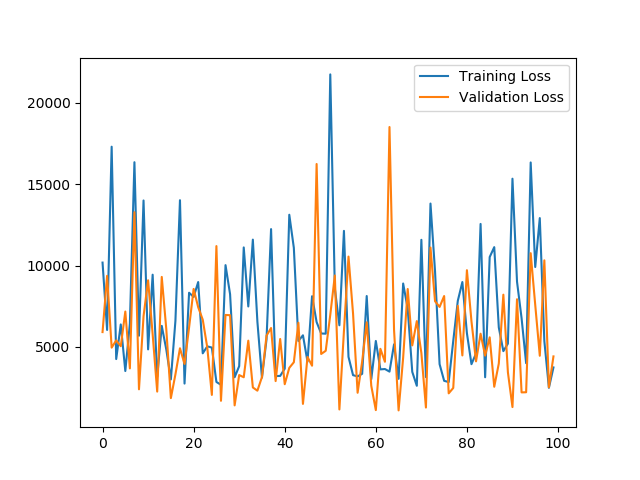
\includegraphics[width=\textwidth]{{Part1/chapter2/chapter/figs/lr0.01net_size16batch2epochs100}.png}
\caption{}
\label{fig.min_batch}
\end{subfigure}%
\qquad
\begin{subfigure}{0.45\textwidth}
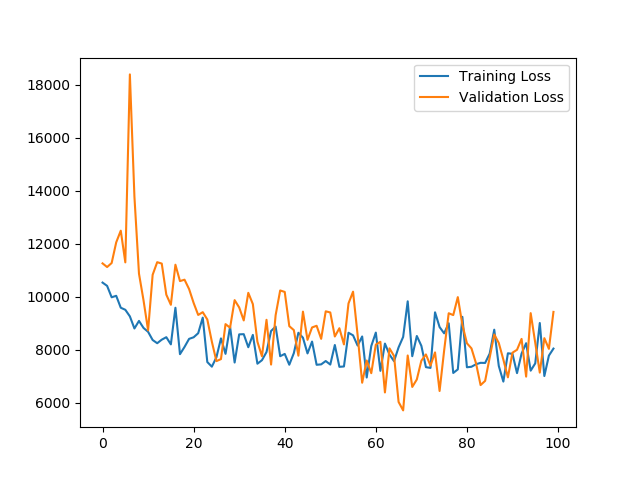
\includegraphics[width=\textwidth]{{Part1/chapter2/chapter/figs/lr0.01net_size16batch128epochs100}.png}
\caption{}
\label{fig.max_batch}
\end{subfigure}
\caption[Effect of differing the size of the batch]{Effect of differing the size of the batch. (a) Small batch size results in large fluctuations between each epoch (b)Large batch size reduces the fluctuations and stabilises the learning rate after each epoch.}
\label{fig.batch_size_comparison}
\end{figure}


\section{Performance}
A large part of determining what architecture to choose and what size images to feed into a CNN is the resources available. Fortunately, this project has been able to make use of the University of Edinburgh's High-performance computing cluster (\cite{ecdf19}). This allowed for training to be implemented on multiple GPUs to reduce the computation time. Being able to implement the training on GPUs was one of the factors that determined which library should be utilised to complete this project.
\subsection{Available Packages}
The two most popular libraries being used by researchers and professionals are Tensorflow and Pytorch. Tensorflow is based on Theano and developed by Google whereas Pytorch is based on Torch and developed by Facebook.
\begin{figure}[htpb]
    \centering
    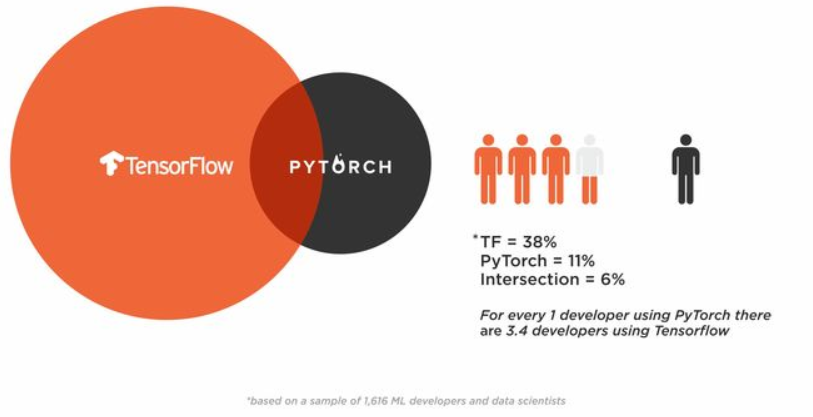
\includegraphics[width=\textwidth]{\dir/figs/tenvspy.PNG}
    \caption[TensorFlow versus PyTorch Usage]{Compares the number of Machine Learning Developers and Data Scientists that use TensorFlow over PyTorch. Based on a sample of 1616 users, data from January 2019 (\cite{Rosenzvaig19}). }.
    \label{fig.tfvspy}
\end{figure}
The main difference is that Tensorflow defines the computational graph for the model before the machine learning model is run. Whereas, PyTorch is dynamic and allows the user to adjust the graph as training progresses. Pytorch is built on top of Numpy and is more pythonic and intuitive. It is easier to implement as it is a lighter framework, which makes it scaleable to multiple GPUs to reduce processing time.
\par
PyTorch was used for this study as it allows for greater customisation when designing how the network reads the training data. Using Pytorch it was possible to design a custom dataloader that was able to perform transformations on two datasets simultaneously (RGB images, and ground truth labels). Additionally, PyTorch uses declarative data parallelism:  \texttt{torch.nn.DataParallel} will wrap any module and it will be parallelised over the batch dimension. This means the network can be trained using GPUs with little effort. The data parallelism also meant that the network could be trained on a GPU and then evaluated on a CPU as Pytorch can adjust the identifiers within the saved model depending on whether or not GPUs are available. More detail on how the dataloader was implemented can be found in \citet{Richmond19b}.